[47 v\textsuperscript{o}] firmata est, utrinque incumbit portatricibus, ut ita non major potentia superanda sit aeri, quam quantum est movere in plano horizontali pon-\pend\pstart\noindent dus illorum quatuor simul sumtorum, et minor etiam sufficit, ob \edtext{tenuitatem,}{\lemma{ob}\Afootnote{ \textit{ (1) }\ figuram tenuissimam \textit{ (2) }\ tenuitatem, \textit{ L}}} et pinnas velorum instar aeri recipiendo accommodatas. Illud notandum est portatrices ita comparatos esse debere, ut malleolo lineam serratam pulsante aliquantulum cedant, et malleolo resurgente restituantur, quod fiat pondere superius iis contraposito. Praeterea ut malleolus impingere possit in lineam serratam a portatoribus demissam, parietes \edtext{vel cancelli, intra quos descendit}{\lemma{parietes}\Afootnote{ \textit{ (1) }\ duo intra quos descen \textit{ (2) }\ vel cancelli, intra quos descendit \textit{ L}}} Linea Serrata versus tabulam non multum progrediantur. \pend \pstart Si, quod non spero aer machinae circumagendae sit insufficiens, erunt tamen omnia in vado. Idem certissime aqua praestiterit. Sit ergo infra Camera quaedam foramen non ante et post, sed in dextro et sinistro habens. Intra eandem Cameram sit alia, habens foramen versus anterius et posterius, ne \edtext{enim}{\lemma{}\Afootnote{enim \textit{ erg.} \textit{ L}}} aquae externae impetus penetret in interiora mutanda foramina. Nam si fluctus a latere veniat secunda camera eludet, si ante vel post, prima. Potest et esse 3\textsuperscript{tia} intra secundam, habens rursus foramen ut primam, ob majorem securitatem. Intra hanc tertiam Cameram, Camerae ex ligno fortissimo sit Camera Rotae\protect\index{Sachverzeichnis}{rota} pinnatae. Ad hanc non sit aditus nisi per angustissimum foramen, et tubum post foramen valde flexum contortumque, et intra tubum rursus aliud foramen et novus tubus. Foramina Tuborum sint instar punctiones aciculae. Tubi ipsi aerei similiter Camera Rotae\protect\index{Sachverzeichnis}{rota} et Rota\protect\index{Sachverzeichnis}{rota}. \edtext{Eadem sit facies aversa, ita ut contorsiones tuborum in oppositum eant.}{\lemma{}\Afootnote{Eadem [...] eant. \textit{ erg.} \textit{ L}}} Ita jam Tubi cum camera rotae\protect\index{Sachverzeichnis}{rota} impleantur aqua, quod ob angustiam foraminum non aliter fiet nisi ut Aeolipilam\protect\index{Sachverzeichnis}{aeolipilae} implemus admotam igni et ita calidam aquae impositam. Semel impleta Camera Rotae\protect\index{Sachverzeichnis}{rota} cum Tubis progrediens novam aquam necessario recipiet veterem amittet, et ita intus rotam primam circumaget. Rotae\protect\index{Sachverzeichnis}{rota} a latere acumen inserat Rota\protect\index{Sachverzeichnis}{rota} media horizonti parallela. Ea circumagat columnam sursum euntem, ibi similis rota\protect\index{Sachverzeichnis}{rota} horizonti parallela, quae lateralem sibi aliam horizonti rectam circumaget, et haec 4\textsuperscript{ta} rota \protect\index{Sachverzeichnis}{rota} erit cum rota\protect\index{Sachverzeichnis}{rota} simplice in machina aerea caetera possunt esse eadem. Nisi, quia hic verendum non est ne machina ad circumagendum nimis gravis fiat, poterit retineri linea simplex supra serratam in qua acicula impactoria firma sit, quamque lineam feriant duo malleoli, ut initio describebatur.\pend \pstart Etsi igitur Aer vadimonium desereret, haberemus tamen nihilominus planissima omnia per aquam in mari, terram in terra. Nam nudae rotae\protect\index{Sachverzeichnis}{rota} curulis ope in terris similiter eadem delineatio itineris praestari potest.\pend \pstart Ut cuilibet manifestum, perfectum igitur instrumentum habemus, etsi non negem, aereum quasi elegantius, subtilius, universalius fore; sed incertius, infirmius magis mutationibus obnoxium. Hoc igitur instrumentum est plus quam Pantometrum\protect\index{Sachverzeichnis}{pantometrum}. Ego quia ipsummet delineat, \pgrk{A>ut'ometron} vocandum \edlabel{censeostart}censeo.\pend \pstart 
   \begin{wrapfigure}{l}{0.5\textwidth}          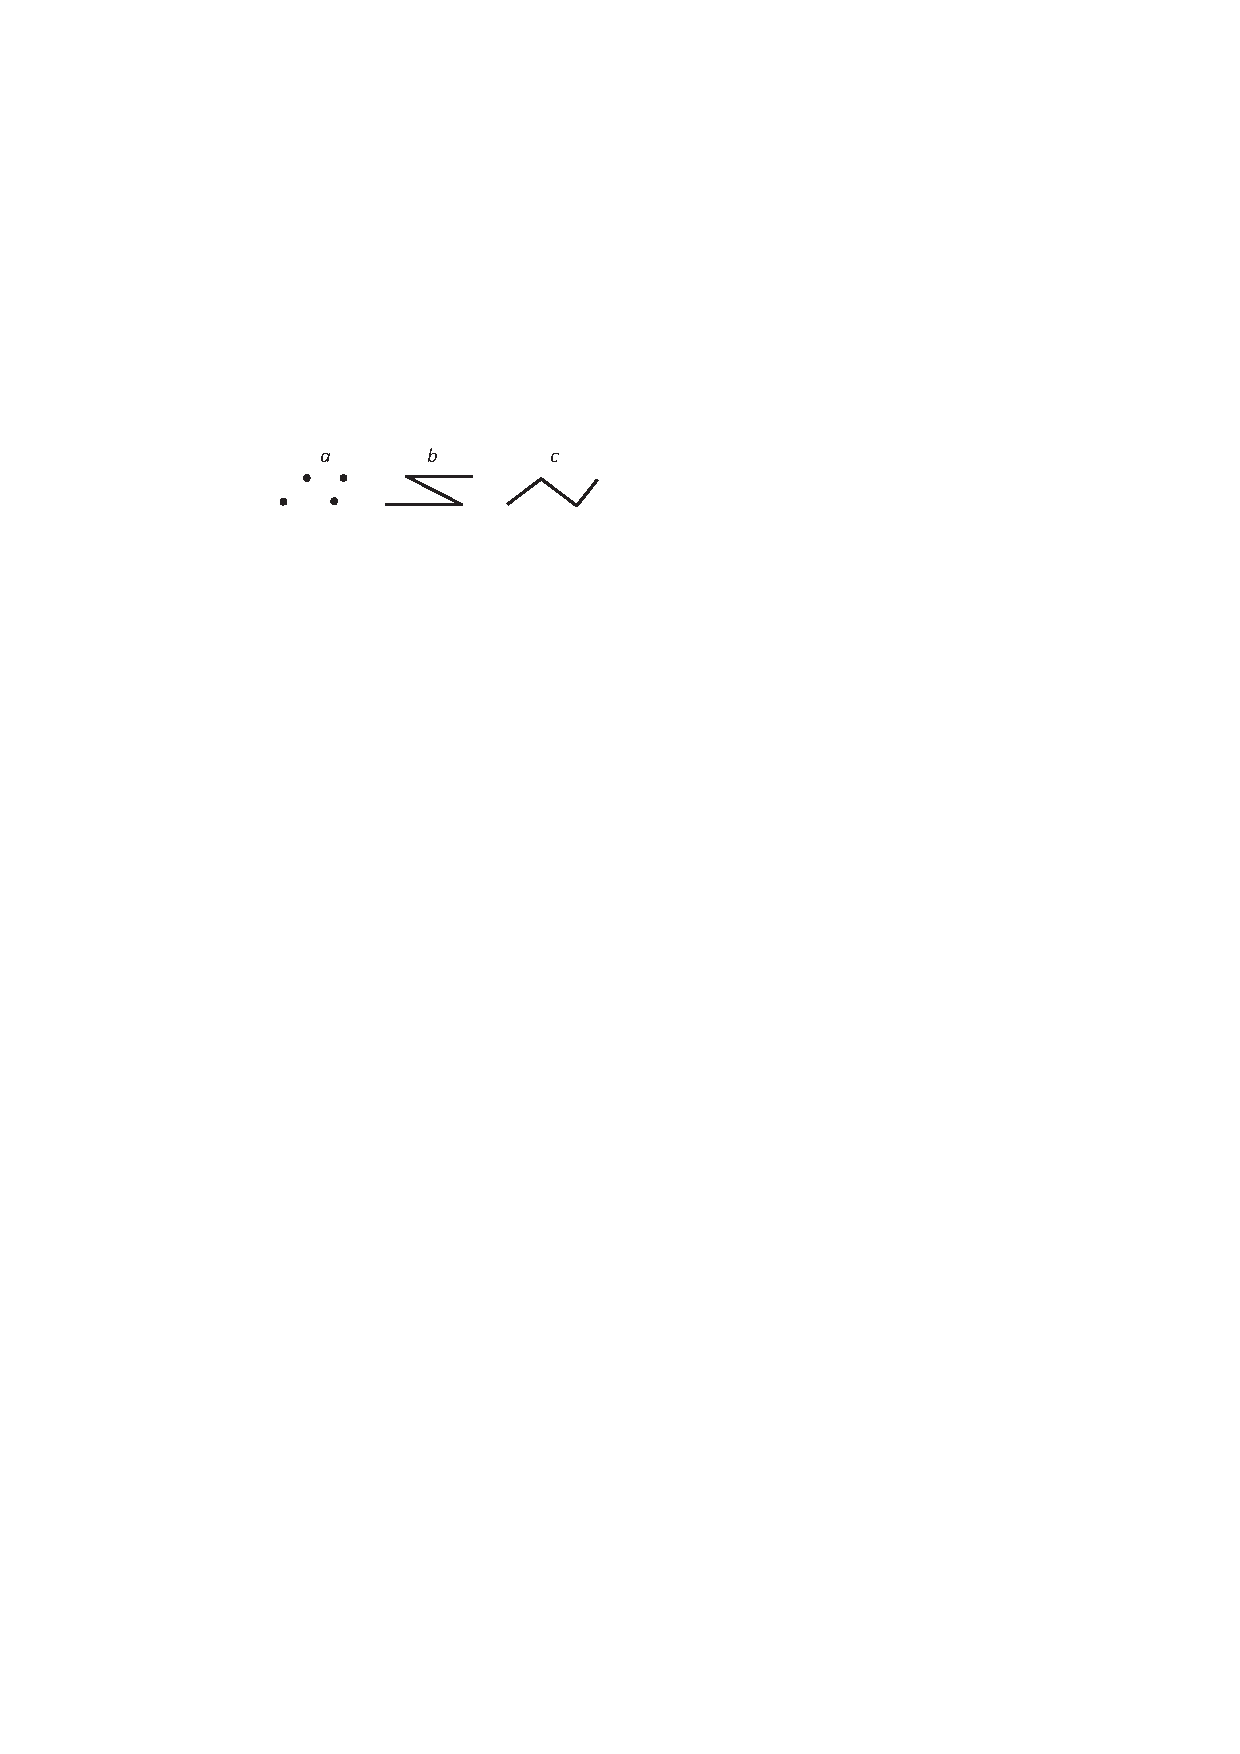
\includegraphics[width=0.4\textwidth]{images/35_15_6_48r1}
   \\\centering\textit{[Fig. 1]}
   \end{wrapfigure}
\edtext{\textit{Exegi monumentum aere} \edtext{\textit{perennius.}\edlabel{censeoend}}{\lemma{\textit{perennius}.}\Bfootnote{\textsc{Horaz}, \cite{00122}\textit{Carmen} III, 30, Vers 1. \hspace{8mm}26 \hspace{3mm}Morino:\hspace{3mm} \textsc{J. Morin}, \cite{00080}\textit{Longitudinum terrestrium Scientia}, Paris 1634.}}}{\lemma{censeo.}\xxref{censeostart}{censeoend}\Afootnote{ \textit{ (1) }\ 
Jamque \textit{ (2) }\ \textit{Exegi monumentum aere perennius.} \textit{ L}}}